\documentclass{aa}

\usepackage{graphicx}
%\usepackage[options]{natbib}
\usepackage{txfonts}
\usepackage{hyperref}
\usepackage{xcolor}
\usepackage{float}           % set colors

\hypersetup{ % this is just my personal choice, feel free to change things
    colorlinks,
    linkcolor={red!50!black},
    citecolor={blue!50!black},
    urlcolor={blue!80!black}}



\begin{document} 

   \title{Temporary title: CMB power spectrum...}

   \author{J. A. Glenndal}

   \institute{Institute of Theoretical Astrophysics,  
                University of Oslo,  0315 Oslo,  Norway\\
              \email{j.a.glenndal@astro.uio.no}
             }

   \date{}

  \abstract{An abstract for the paper. Describe the paper. What is the paper about, what are the main results, etc.}

   \keywords{   cosmic microwave background  --
                large-scale structure of Universe
               }

   \maketitle

\section{Introduction}
Write an introduction here. Give context to the paper. Citations to relevant papers. You only need to do this in the end for the last milestone.

\section{Milestone I}
%Some introduction about what it is all about.
In this milestone we will look at the expansion history of a homogeneous and isotropic universe governed by the well known Friedmann equation \ref{Friedmann}.
The universe we consider consists of baryonic matter ($\Omega_b$), cold dark matter ($\Omega_\mathrm{CDM}$), radiation ($\Omega_\gamma$), neutrinos ($\Omega_\nu$)
and dark energy ($\Omega_\Lambda$), where $\Omega$ is the mass/energy density divided by the critical density ($\rho_c = 3H^2/8\pi G$).\\
\\
Since our universe is approximately homogeneous and isotropic on large scales, the solution we calculate will be  



Since our goal in the end is to study the
cosmic microwave background (CMB), the homogeneous solution of the universe is of great interest. This is because the CMB is close to
being homogeneous with perturbations of order $10^{-5}$.
     


\subsection{Theory}
%The theory behind this milestone.
The parameters we use for our universe are given below.
%\vspace*{-1.5cm}

\begin{equation}
      \boxed{
   \begin{aligned}
      h &= 0.67, \\
      T_{\rm CMB 0} &= 2.7255\,K, \\
      N_{\rm eff} &= 3.046, \\
      \Omega_{\rm b 0} &= 0.05, \\
      \Omega_{\rm CDM 0} &= 0.267,\\
      \Omega_{k 0} &= 0, \\
      \Omega_{\nu 0} &= N_{\rm eff}\cdot \frac{7}{8}\left(\frac{4}{11}\right)^{4/3}\Omega_{\gamma 0}, \\
      \Omega_{\gamma 0} &= 2\cdot \frac{\pi^2}{30} \frac{(k_bT_{\rm CMB 0})^4}{\hbar^3 c^5} \cdot \frac{8\pi G}{3H_0^2},\\
      \Omega_{\Lambda 0} &= 1 - (\Omega_{k 0}+\Omega_{b 0}+\Omega_{\rm CDM 0}+\Omega_{\gamma 0}+\Omega_{\nu 0}),
   \end{aligned}}
\end{equation}

\vspace*{0.3cm}
\noindent
where the subscript 0 denotes today's value. $h$ is the dimensionless Hubble constant. More details can be found at \cite{winther:2023}. \\ \\

\noindent
The Friedmann equation is given by
\begin{equation}\label{Friedmann}
      H = H_0 \sqrt{(\Omega_{b0}+\Omega_{\rm CDM 0})a^{-3} + (\Omega_{\gamma 0} + \Omega_{\nu 0}) a^{-4} + \Omega_{k 0} a^{-2} + \Omega_{\Lambda 0}},
\end{equation}
where $a$ is the scale factor and  $H = \frac{\dot{a}}{a}$. We will not use cosmic time ($t$) as our time variable.
Instead, we use $x=\ln a$ as our dimensionless time variable. This implies that $a = e^x$ for conversion. Since $a(t=0)=0$ and $a(t=t_0)=1$
we get $t=0 \iff x = -\infty$ and $t=t_0 \iff x = 0$. The cosmic time as a function of $x$ be found from the differential equation 
\begin{equation}\label{cosmic_time_differential_equation}
      \frac{dt}{dx} = \frac{1}{H},
\end{equation}
which can be solved numerically. \\ \\
\noindent
We also use a scaled Hubble parameter defined by $\mathcal{H}\equiv aH$
The evolution of the $\Omega$s can be expressed as a function of $a$ as showed below. 
\begin{equation}
      \hspace*{2cm}
   \begin{aligned}
      \Omega_{k}(a) &= \frac{\Omega_{k0}}{a^2H(a)^2/H_0^2}\\
      \Omega_{\rm CDM}(a) &= \frac{\Omega_{\rm CDM 0}}{a^3H(a)^2/H_0^2} \\
      \Omega_b(a) &= \frac{\Omega_{b 0}}{a^3H(a)^2/H_0^2} \\
      \Omega_\gamma(a) &= \frac{\Omega_{\gamma 0}}{a^4H(a)^2/H_0^2} \\
      \Omega_{\nu}(a) &= \frac{\Omega_{\nu 0}}{a^4H(a)^2/H_0^2} \\
      \Omega_{\Lambda}(a) &= \frac{\Omega_{\Lambda 0}}{H(a)^2/H_0^2}.
   \end{aligned}
\end{equation}


\subsection{Implementation details}
Something about the numerical work.

\subsection{Results}
Show and discuss the results.

\section{Milestone II}
Some introduction about what it is all about.

\subsection{Theory}
The theory behind this milestone.

\subsection{Implementation details}
Something about the numerical work.

\subsection{Results}
Show and discuss the results.


%3333333333333333333333333333333333333333333333333333333333333333333333333333333333333333333333333333333333333333333333333333333333333333333333333333333
%3333333333333333333333333333333333333333333333333333333333333333333333333333333333333333333333333333333333333333333333333333333333333333333333333333333
%3333333333333333333333333333333333333333333333333333333333333333333333333333333333333333333333333333333333333333333333333333333333333333333333333333333
\section{Milestone III}
Some introduction about what it is all about.
%In this milestone we look at 
In this milestone we calculate the evolution of the structures in the universe. In practice, this is done by 
solving the perturbed Einstein-Boltzmann equations numerically.
\\
\\
We have used linear perturbation theory to perturb the Einstein-Boltzmann equations. Easier to solve in Fourier space. Energy perturbations influence the
metric perturbations through the Einstein equations. We use the Newtonian gauge for the perturbed metric

In order to determine how structures form in the universe, we can perturb




We have evolved perturbations in time and studyed their time evolution at different scales. When instead
looking at one time and all scales we get a power spectrum, I think... or maybe not...


\subsection{Theory}
%The theory behind this milestone.
\\
\\
%Boltzmann equations, spherical harmonics, perturbation theory...
Linearized Einstein and Boltzmann equations for perturbed distribution functions.





\subsection{Implementation details}
Something about the numerical work.

\subsection{Results}
\subsubsection{Test results}
The code produces the following results with the cosmological test parameters given in table \ref{tab:test_parameters}. All the figures show plots at three different scales.
In figures \ref{fig:test1} and \ref{fig:test2} we see the overdensity and the velocity, respectively, for both CDM and baryons. In figures \ref{fig:test3}
and \ref{fig:test4} we see the photon temperature monopole, $\Theta_0$, and the photon temperature dipole, $\Theta_1$, respectively. The gravitational potential, $\Phi$, is plotted
in figure \ref{fig:test5}. All plots seem to agree with the plots produced by \cite{winther:2023}.   


\begin{table}[h!] %%h! er for å tvinge tabellen til å være nærmest mulig her i dokumentet
   %\begin{center}
     \caption{Cosmological test parameters.} %Tabelltekst
     \label{tab:test_parameters}
     \begin{tabular}{l|l}%|r} % for hver kolonne har du {a|b|c} der a er for 1.kolonne, b for 2. kolonne etc, l=venstrestil, r=høyrestilt, c = senterstilt. Se posisjonen til tallene i de forskjellige kolonnene. Har du 4 kolonner der alle er senterstilt blir det f.eks. {c|c|c|c}
       \textbf{Parameter} & \textbf{Value}\\% & \textbf{Unit}\\ %innhold i hver kolonne, legg til flere her hvis du har flere kolonner
       %(i) & (m) & (m/s)\\ %enheter for hver kolonne
       \hline %en horisontall linje for å skille overskriften fra tallene under. Vil du ha en slik linje mellom hver rad i tabellen så legg til en \hline mellom hver rad nedover her. Merk \\ er som vanlig linjeskift mens & skiller kolonner
       $h$ & 0.7\\
       $\Omega_\mathrm{b}$ & 0.05\\
       $\Omega_\mathrm{CDM}$& 0.45\\
       $\Omega_\mathrm{\Lambda}$ & 0.5\\
       $\Omega_\mathrm{k}  $     & 0\\
       $\Omega_\mathrm{\nu}$ & 0\\
       $T_\mathrm{CMB}$ & 2.7255 $[K]$\\
       %$Y_\mathrm{p}$ & 0\\
       \hline
     \end{tabular}
   %\end{center}
 \end{table}

\begin{figure}[h!]
   %\hspace{-0.48cm}   
   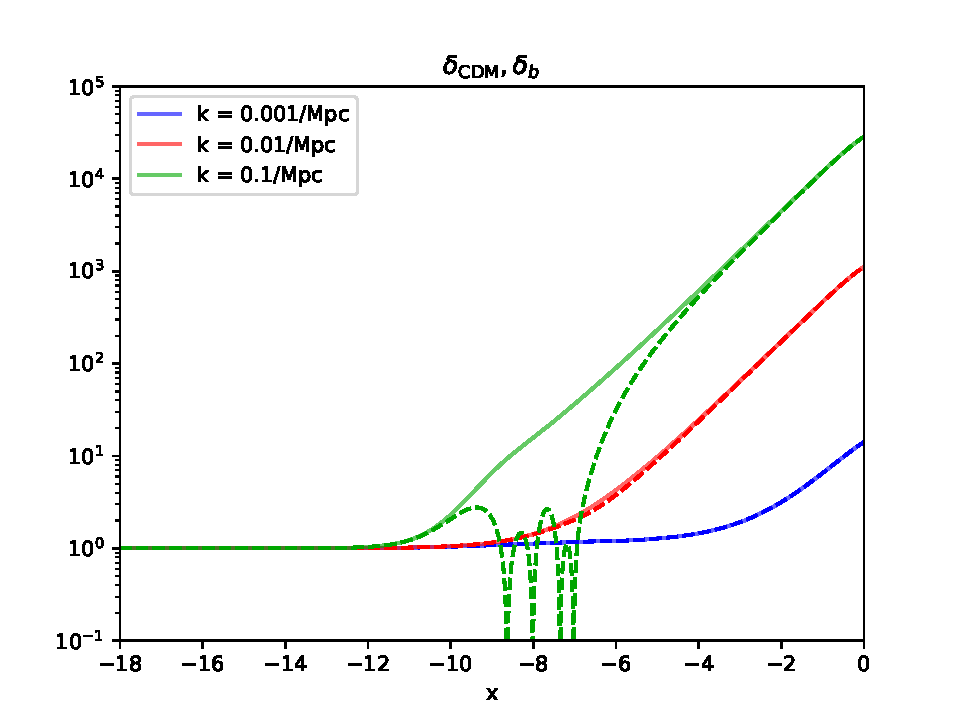
\includegraphics[scale=0.6]{../figures/milestone3/test_delta_cdm_delta_b.pdf}
   \caption{The CDM overdensities, in solid lines, and the absolute value of the baryon overdensities,
    in dotted lines, are plotted at different scales, $k$.}\label{fig:test1}
\end{figure}

\begin{figure}[h!]
   %\hspace{-0.48cm}   
   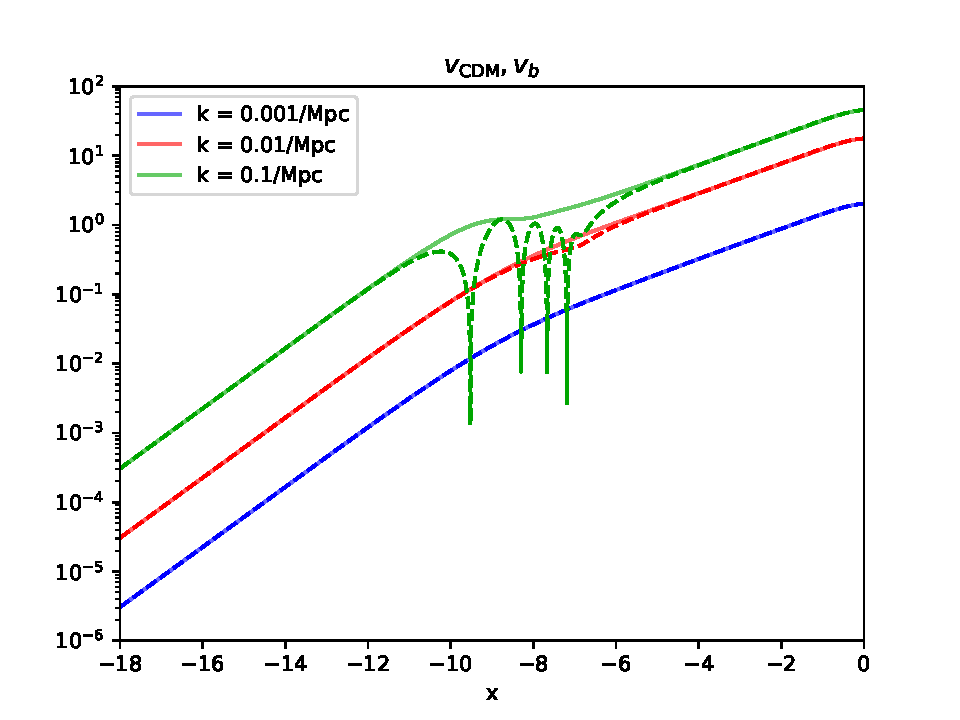
\includegraphics[scale=0.6]{../figures/milestone3/test_v_cdm_v_b.pdf}
   \caption{The CDM velocities, in solid lines, and the absolute value of the baryon velocities,
    in dotted lines, are plotted at different scales, $k$.}\label{fig:test2}
\end{figure}


\begin{figure}[h!]
   %\hspace{-0.48cm}   
   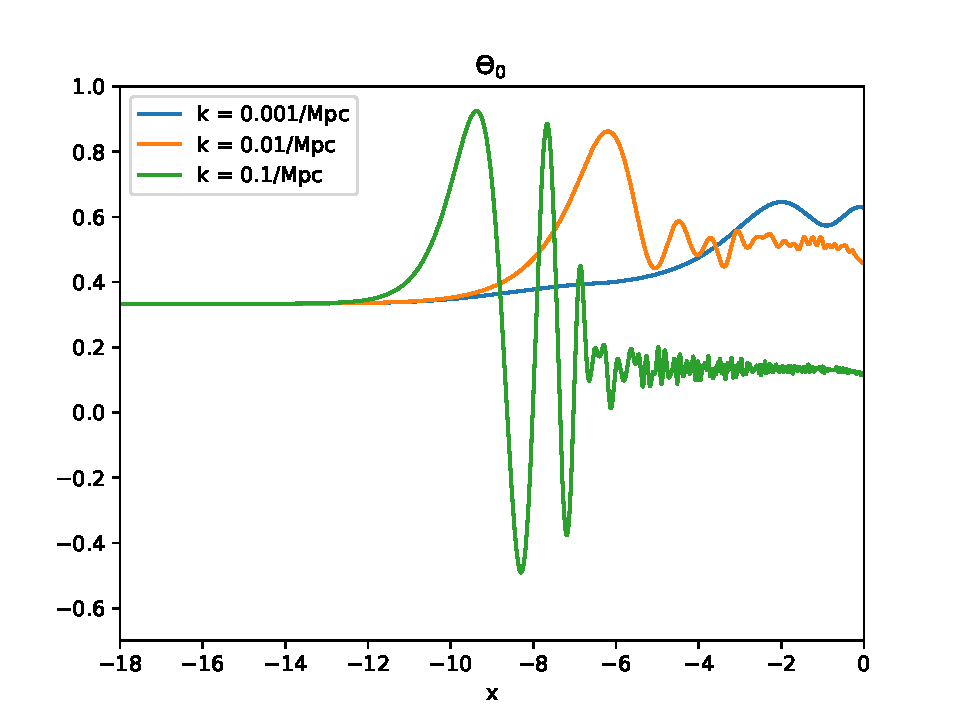
\includegraphics[scale=0.6]{../figures/milestone3/test_theta_0.pdf}
   \caption{The photon temperature monopole at different scales, $k$.}\label{fig:test3}
\end{figure}

\begin{figure}[h!]
   %\hspace{-0.48cm}   
   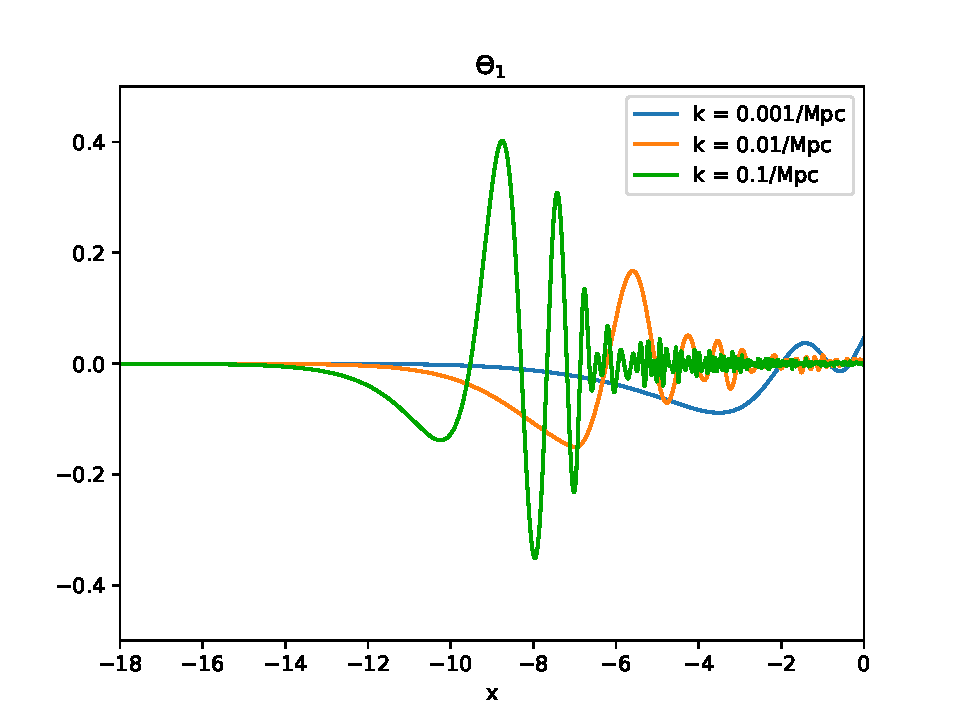
\includegraphics[scale=0.6]{../figures/milestone3/test_theta_1.pdf}
   \caption{The photon temperature dipole at different scales, $k$.}\label{fig:test4}
\end{figure}

\begin{figure}[h!]
   %\hspace{-0.48cm}   
   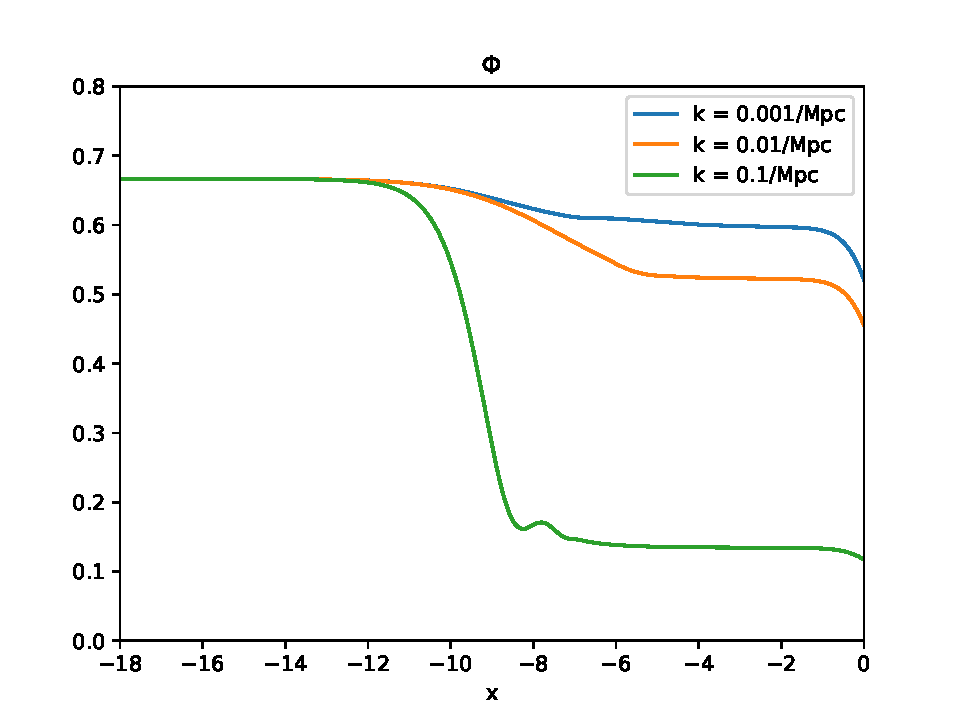
\includegraphics[scale=0.6]{../figures/milestone3/test_phi.pdf}
   \caption{The gravitational potential at different scales, $k$.}\label{fig:test5}
\end{figure}

\subsubsection{Results}
%theory section maybe???
% write about the slope of delta_cdm and compare to analytical result...all plots in general
Gravity travels with the same velocity as light. Therefore, the conformal time, $\eta$, gives us the maximum reach of gravity, e.g. if $\eta= 1$ Mpc we know that 
scales up to 1 Mpc will cluster due to gravity. This is also reflected in our results, hopefully...  
%Show and discuss the results.

\begin{figure}[h!]
   %\hspace{-0.48cm}   
   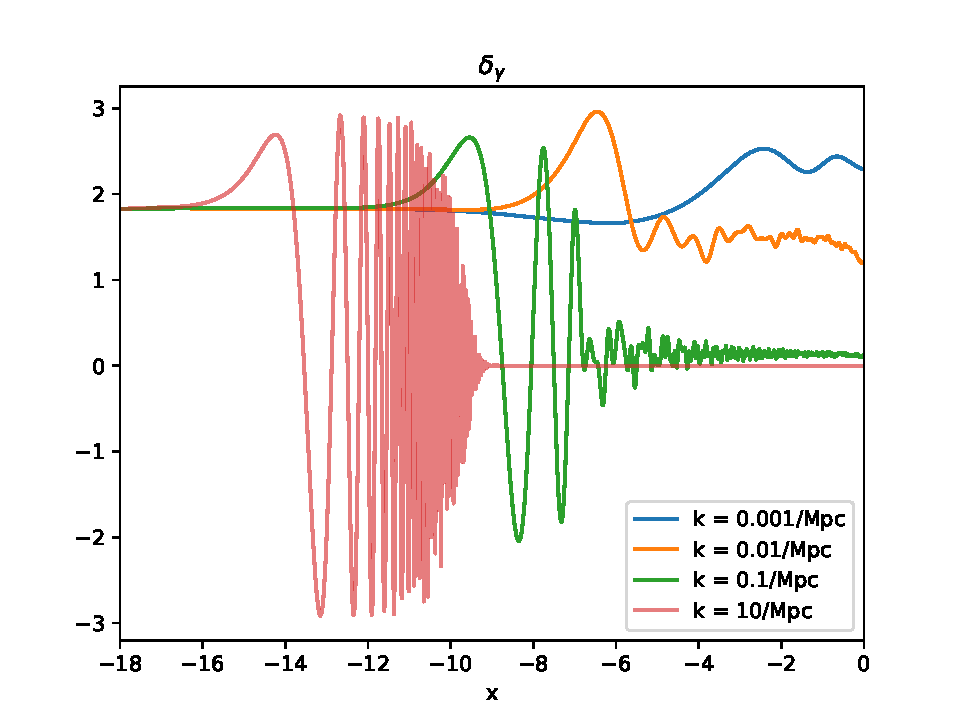
\includegraphics[scale=0.6]{../figures/milestone3/delta_gamma.pdf}
   \caption{The photon density perturbation, $\delta_\gamma = 4\Theta_0$, at four different scales, $k$. }\label{fig:delta_gamma}
\end{figure}

\begin{figure}[h!]
   %\hspace{-0.48cm}   
   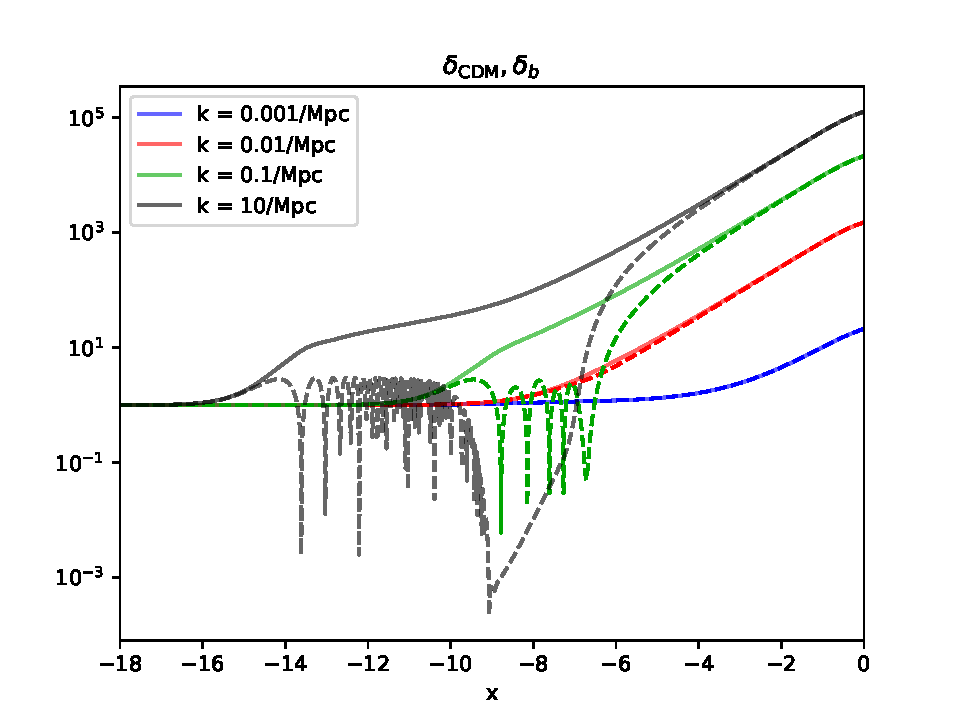
\includegraphics[scale=0.6]{../figures/milestone3/delta_cdm_delta_b.pdf}
   \caption{The CDM overdensity and the absolute value of the baryon overdensity plotted at four different scales, $k$. The solid lines are for CDM and the dotted lines are for baryons.}\label{fig:delta_cdm_delta_b}
\end{figure}

\begin{figure}[h!]
   %\hspace{-0.48cm}   
   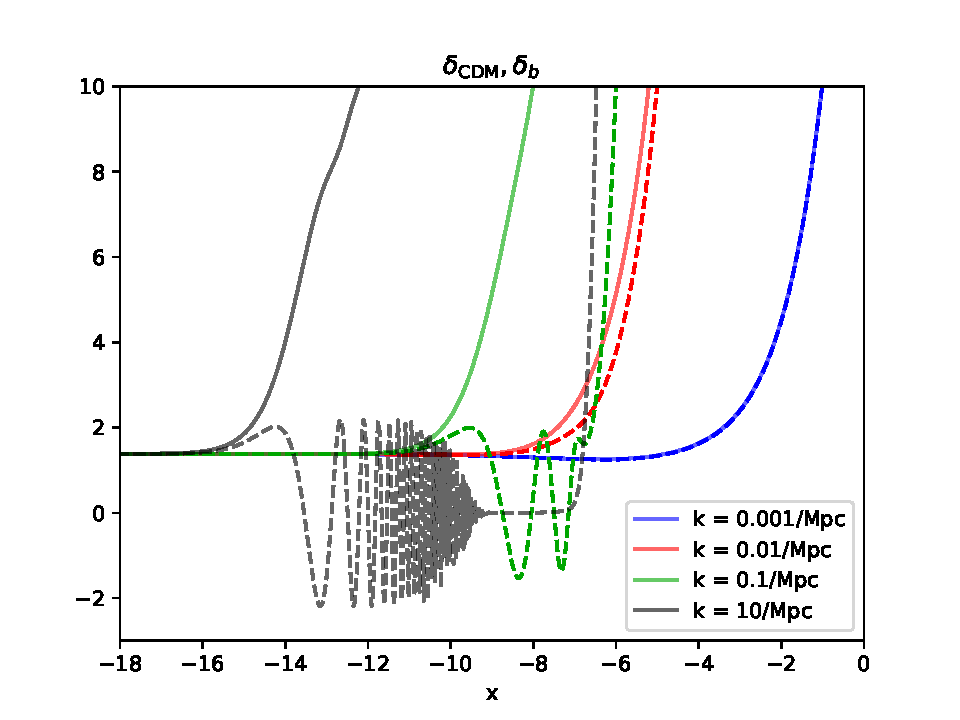
\includegraphics[scale=0.65]{../figures/milestone3/delta_cdm_delta_b_zoom.pdf}
   \caption{A closer look at figure \ref{fig:delta_cdm_delta_b} with linear y-scale and with the correct sign for the baryon overdensity.}\label{fig:delta_cdm_delta_b_zoom}
\end{figure}

\begin{figure}[h!]
   %\hspace{-0.48cm}   
   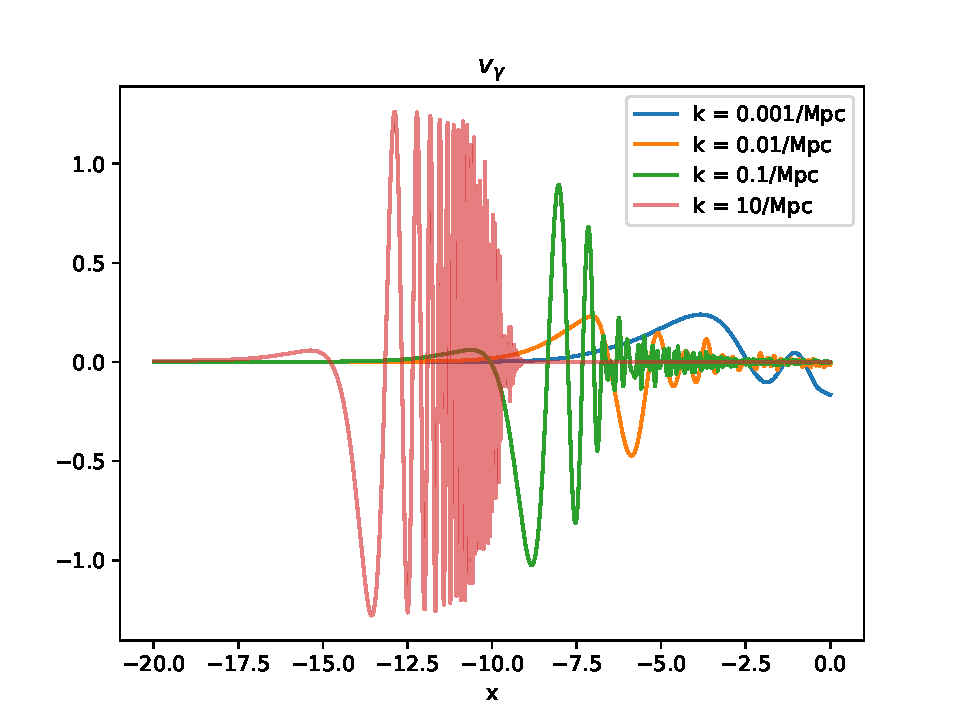
\includegraphics[scale=0.6]{../figures/milestone3/v_gamma.pdf}
   \caption{The photon velocity perturbation, $v_\gamma=-3\Theta_1$, at four different scales, $k$.}\label{fig:v_gamma}
\end{figure}

\begin{figure}[h!]
   %\hspace{-0.48cm}   
   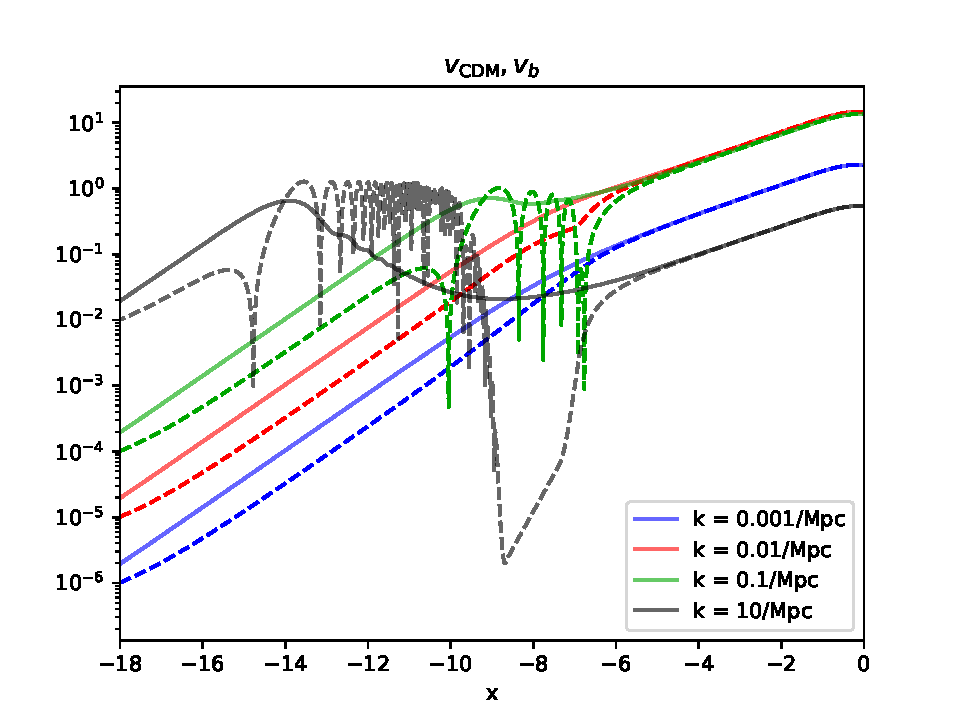
\includegraphics[scale=0.6]{../figures/milestone3/v_cdm_v_b.pdf}
   \caption{The CDM velocities, in solid lines, and the absolute value of the baryon velocities,
   in dotted lines, are plotted at four different scales, $k$.}\label{fig:v_cdm_v_b}
\end{figure}

\begin{figure}[h!]
   %\hspace{-0.48cm}   
   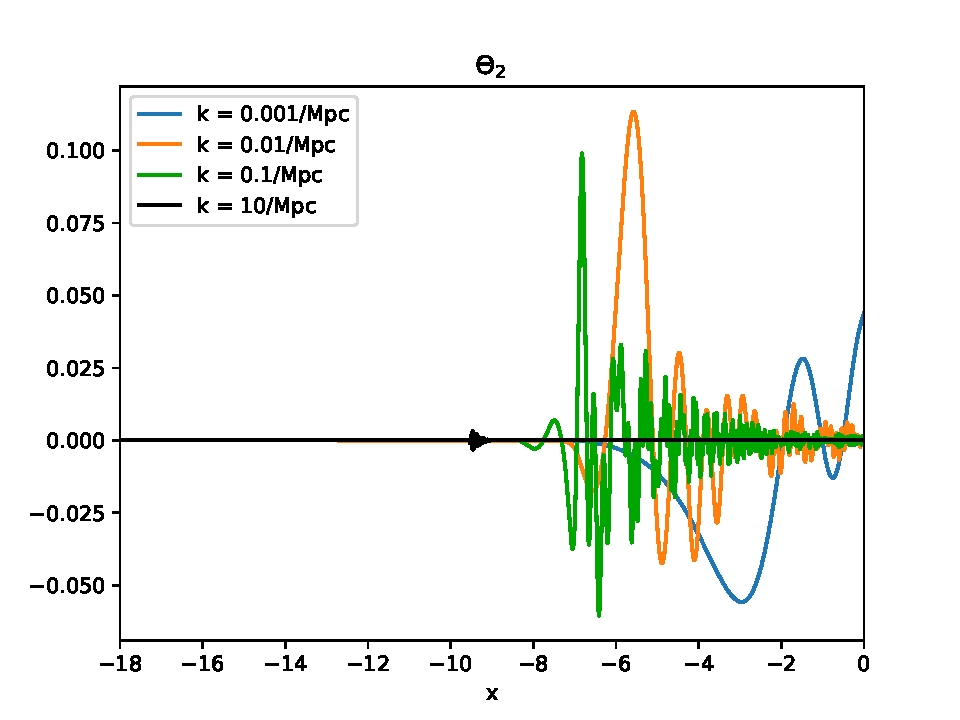
\includegraphics[scale=0.65]{../figures/milestone3/theta_2.pdf}
   \caption{The photon temperature quadrupole, $\Theta_2$, at four different scales, $k$.}\label{fig:theta2}
\end{figure}

\begin{figure}[h!]
   %\hspace{-0.48cm}   
   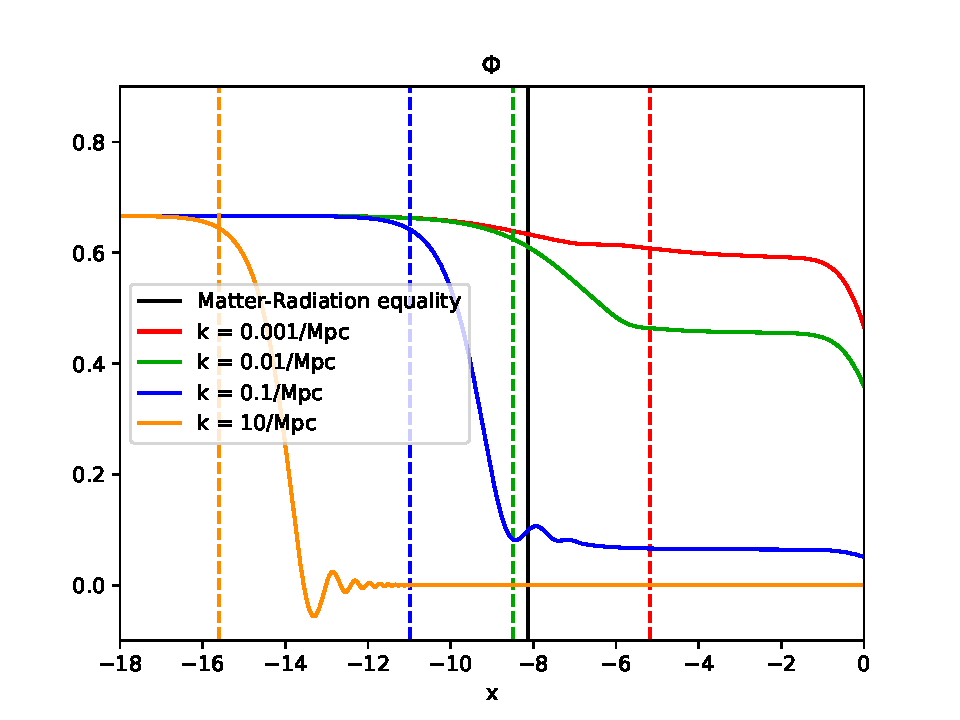
\includegraphics[scale=0.6]{../figures/milestone3/phi.pdf}
   \caption{The gravitational potential at four different scales, $k$.}\label{fig:phi}
\end{figure}

\begin{figure}[h!]
   %\hspace{-0.48cm}   
   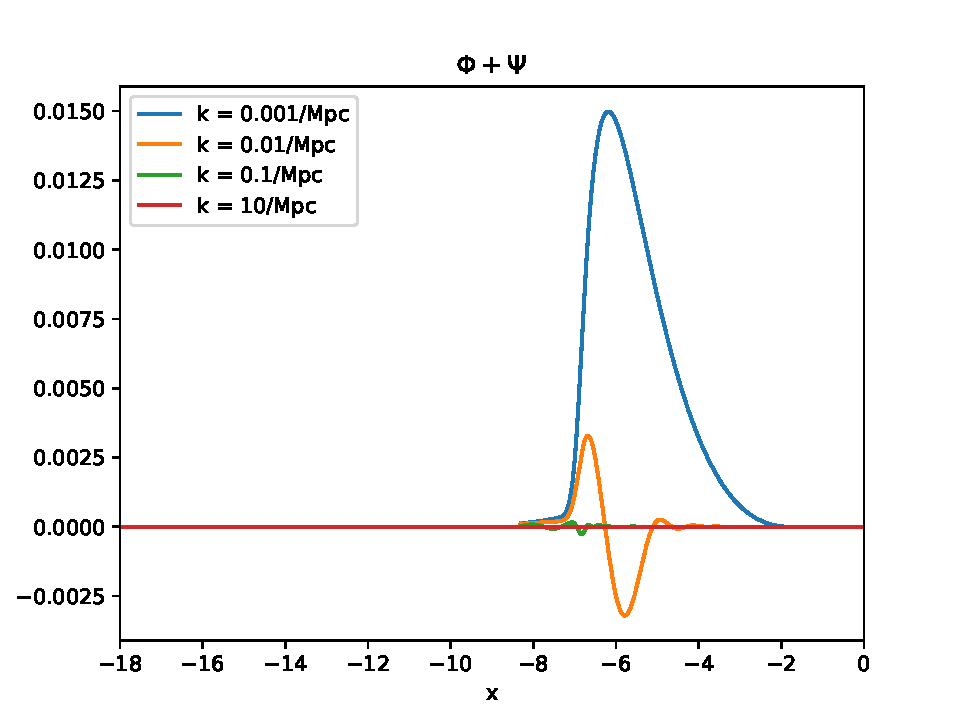
\includegraphics[scale=0.6]{../figures/milestone3/phi_psi.pdf}
   \caption{The sum of the two gravitational potentials, $\Phi$ and $\Psi$, at four different scales, $k$.}\label{fig:phi_psi}
\end{figure}



\section{Milestone IV}
Some introduction about what it is all about.

\subsection{Theory}
The theory behind this milestone.

\subsection{Implementation details}
Something about the numerical work.

\subsection{Results}
Show and discuss the results.

\section{Conclusions}

Write a short summary and conclusion in the end. 

%\begin{acknowledgements}
%      I thank my mom for financial support!!!
%\end{acknowledgements}

\bibliographystyle{aa} % style aa.bst
\bibliography{refs} % your references Yourfile.bib
%

%\bibliographystyle{plain} % We choose the "plain" reference style
%\section*{References}
%\bibliography{refs} % Entries are in the refs.bib file

%\begin{thebibliography}{}
%      \bibitem[1966]{baker} Baker, N. 1966,
%      in Stellar Evolution,
%      ed.\ R. F. Stein,\& A. G. W. Cameron
%      (Plenum, New York) 333
%
%      \bibitem[2023]{winther} Winther, H.A. 2023,
%      %\href{https://cmb.wintherscoming.no/milestone1.php}
%\end{thebibliography}

\end{document}